\documentclass[12pt]{article}
\usepackage[a4paper, margin=2cm]{geometry}
\usepackage[utf8]{inputenc}
\usepackage{indentfirst}
\usepackage{enumitem}
\usepackage{fancyhdr}
\usepackage{amsmath}
\usepackage{mdframed}
\usepackage{xcolor}
\usepackage{listings}
\usepackage{tikz}
\usetikzlibrary{shapes.geometric, arrows}

\lstset{
    language=Java,
    basicstyle=\ttfamily\small,
    keywordstyle=\color{blue},
    commentstyle=\color{gray},
    stringstyle=\color{red},
    numbers=left,
    numberstyle=\tiny,
    stepnumber=1,
    numbersep=5pt,
    backgroundcolor=\color{white},
    showspaces=false,
    showstringspaces=false,
    showtabs=false,
    frame=single,
    tabsize=2,
    captionpos=b,
    breaklines=true,
    breakatwhitespace=true,
    escapeinside={\%*}{*)}
}

\renewcommand{\thesection}{Soal \arabic{section}}

\pagestyle{fancy}
\fancyhf{}
\rhead{TUGAS PRAKTIKUM ALPRO 1}
\lhead{BAB 10}
\rfoot{Halaman \thepage}

\title{TUGAS PRAKTIKUM ALGORITMA DAN PEMROGRAMAN 1}
\author{}
\date{Pertemuan ke-8\\BAB 10: Array\\Deadline: 17 November 2024 Pukul 18:29}

\begin{document}

\maketitle
\thispagestyle{empty}
\setcounter{page}{0}

\section*{Petunjuk}
\begin{itemize}
    \item Kerjakan semua soal di bawah ini dengan menggunakan bahasa Java.
    \item Implementasikan konsep Array sesuai materi Modul 10.
    \item Program harus dapat di-compile dan di-run tanpa error.
    \item Nama file source code (.java) harus sesuai dengan nama class.
    \item Kumpulkan file source code (.java) untuk setiap program dan laporan praktikum (.pdf).
    \item Source code di dalam laporan wajib dilampirkan menggunakan syntax highlighter.
    \item Format laporan praktikum dapat dilihat di myITS Classroom.
    \item Penamaan file laporan praktikum adalah \texttt{LaporanPraktikum8\_Kelompok1\_Nama Lengkap}.pdf.
    \item Hasil pengerjaan dikumpulkan di myITS Classroom dalam satu file (.zip) dengan nama \texttt{LaporanPraktikum8\_Kelompok1\_Nama Lengkap}.zip yang berisi file source code (.java) dan laporan praktikum (.pdf).
    \item Deadline pengumpulan: \textbf{17 November 2024 Pukul 18:29}
\end{itemize}

\newpage

\section{Implementasi Algoritma Sorting}

Implementasikan algoritma pengurutan ke dalam bahasa Java menggunakan array dengan melengkapi code di bawah ini.

\begin{lstlisting}
import java.util.Scanner;

public class SortingNilai {
    
    // LENGKAPI: Method untuk input nilai
    public static int[] inputNilai(Scanner input) {
        System.out.print("Masukkan jumlah nilai: ");
        int jumlah = input.nextInt();
        int[] array = new int[jumlah];
        
        for (int i = 0; i < jumlah; i++) {
            System.out.print("Masukkan nilai ke-" + (i+1) + ": ");
            // LENGKAPI
        }
        return array;
    }
    
    // LENGKAPI: Method untuk sorting array
    public static void sortingArray(int[] array) {
        for (int i = 0; i < array.length - 1; i++) {
            for (int j = i + 1; j < array.length; j++) {
                // LENGKAPI: Kondisi if dan proses penukaran
                if (/* LENGKAPI */) {
                    // LENGKAPI: Proses penukaran nilai
                }
            }
        }
    }
    
    // LENGKAPI: Method untuk menampilkan array
    public static void tampilkanArray(String pesan, int[] array) {
        // LENGKAPI
    }
    
    public static void main(String[] args) {
        Scanner input = new Scanner(System.in);
        
        // LENGKAPI: Panggil method inputNilai
        int[] array = // LENGKAPI
        
        // LENGKAPI: Panggil method tampilkanArray untuk array sebelum sorting
        // LENGKAPI
        
        // LENGKAPI: Panggil method sortingArray
        // LENGKAPI
        
        // LENGKAPI: Panggil method tampilkanArray untuk array setelah sorting
        // LENGKAPI
    }
}
\end{lstlisting}


\textbf{Contoh Output Program:}
\begin{mdframed}[backgroundcolor=gray!15]
\begin{verbatim}
Masukkan jumlah nilai: 5
Masukkan nilai ke-1: 85
Masukkan nilai ke-2: 92
Masukkan nilai ke-3: 78
Masukkan nilai ke-4: 65
Masukkan nilai ke-5: 90

Array sebelum sorting: [85, 92, 78, 65, 90]
Array setelah sorting: [65, 78, 85, 90, 92]
\end{verbatim}
\end{mdframed}

\textbf{Requirements:}
\begin{itemize}
    \item Jumlah data harus lebih dari 0
    \item Implementasikan algoritma sorting menggunakan method
    \item Buat method untuk input nilai, sorting array, dan menampilkan array
    \item Program menerima input array dari user
    \item Tampilkan array sebelum dan sesudah diurutkan
    \item Gunakan nested loop dalam method sorting
\end{itemize}

\newpage

\section{Sahroni dan Data Nilai Mahasiswa}

\textbf{Sahroni adalah asisten laboratorium} yang bertugas mengelola data nilai praktikum mahasiswa. Bantulah Sahroni membuat program untuk menyimpan dan menganalisis data nilai menggunakan array.

\textbf{Spesifikasi Program:}
\begin{itemize}
    \item Simpan nilai mahasiswa dalam array integer
    \item Hitung rata-rata nilai
    \item Cari nilai tertinggi dan terendah
    \item Tampilkan semua nilai
\end{itemize}

\textbf{Implementasikan flowchart berikut ke dalam bahasa Java:}

\begin{center}
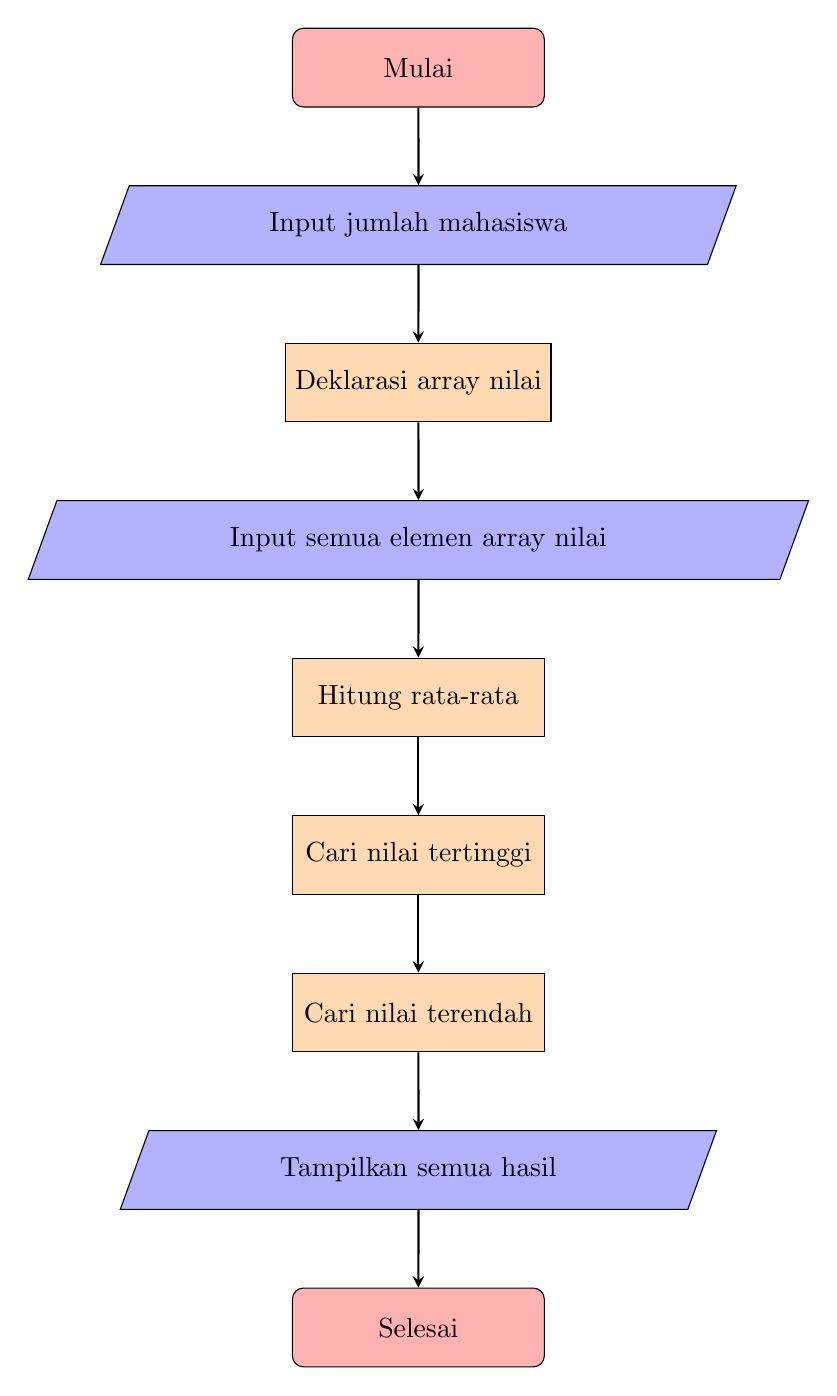
\begin{tikzpicture}[node distance=2cm]
\tikzstyle{startstop} = [rectangle, rounded corners, minimum width=3.2cm, minimum height=1cm, text centered, draw=black, fill=red!30]
\tikzstyle{io} = [trapezium, trapezium left angle=70, trapezium right angle=110, minimum width=3.5cm, minimum height=1cm, text centered, draw=black, fill=blue!30]
\tikzstyle{process} = [rectangle, minimum width=3.2cm, minimum height=1cm, text centered, draw=black, fill=orange!30]
\tikzstyle{arrow} = [thick,->,>=stealth]

\node (start) [startstop] {Mulai};
\node (inputJumlah) [io, below of=start] {Input jumlah mahasiswa};
\node (deklarasi) [process, below of=inputJumlah] {Deklarasi array nilai};
\node (inputArray) [io, below of=deklarasi] {Input semua elemen array nilai};
\node (hitungRata) [process, below of=inputArray] {Hitung rata-rata};
\node (cariMax) [process, below of=hitungRata] {Cari nilai tertinggi};
\node (cariMin) [process, below of=cariMax] {Cari nilai terendah};
\node (output) [io, below of=cariMin] {Tampilkan semua hasil};
\node (stop) [startstop, below of=output] {Selesai};

\draw [arrow] (start) -- (inputJumlah);
\draw [arrow] (inputJumlah) -- (deklarasi);
\draw [arrow] (deklarasi) -- (inputArray);
\draw [arrow] (inputArray) -- (hitungRata);
\draw [arrow] (hitungRata) -- (cariMax);
\draw [arrow] (cariMax) -- (cariMin);
\draw [arrow] (cariMin) -- (output);
\draw [arrow] (output) -- (stop);

\end{tikzpicture}
\end{center}

\newpage
\textbf{Contoh Output:}
\begin{mdframed}[backgroundcolor=gray!15]
\begin{verbatim}
Masukkan jumlah mahasiswa: 4
Nilai mahasiswa 1: 85
Nilai mahasiswa 2: 92
Nilai mahasiswa 3: 78
Nilai mahasiswa 4: 65

=== HASIL ANALISIS ===
Nilai: [85, 92, 78, 65]
Rata-rata: 80.0
Nilai tertinggi: 92
Nilai terendah: 65
\end{verbatim}
\end{mdframed}

\textbf{Requirements:}
\begin{itemize}
    \item Jumlah data harus lebih dari 0
    \item Setiap proses pada flowchart harus diimplementasikan dalam method yang terpisah
    \item Buat method untuk input jumlah mahasiswa, input nilai ke array, menghitung rata-rata, mencari nilai tertinggi, mencari nilai terendah, dan menampilkan hasil
    \item Data nilai harus disimpan dalam array
    \item Output harus sesuai format contoh
\end{itemize}


\end{document}